\documentclass[UTF8]{ctexart}


\usepackage{tikz,mathpazo}
\usetikzlibrary{shapes.geometric, arrows}
\usetikzlibrary{calc}


\usepackage{listings}
%插入代码的配置
\definecolor{mygreen}{rgb}{0,0.6,0}
\definecolor{mygray}{rgb}{0.5,0.5,0.5}
\definecolor{mymauve}{rgb}{0.58,0,0.82}
\lstset{
 backgroundcolor=\color{lightgray},
 basicstyle = \footnotesize,
 breakatwhitespace = false,
 breaklines = true,
 captionpos = b,
 commentstyle = \color{mygreen}\bfseries,
 extendedchars = false,
 frame =shadowbox,
 framerule=0.5pt,
 keepspaces=true,
 keywordstyle=\color{blue}\bfseries, % keyword style
 language = C++,                     % the language of code
 otherkeywords={string},
 numbers=left,
 numbersep=5pt,
 numberstyle=\tiny\color{mygray},
 rulecolor=\color{black},
 showspaces=false,
 showstringspaces=false,
 showtabs=false,
 stepnumber=1,
 stringstyle=\color{mymauve},        % string literal style
 tabsize=2,
 title=\lstname,
 escapeinside=``
}



\usepackage{geometry}
\geometry{left=2cm, right=2cm, top=2cm, bottom=2cm}

%得到引用的标题内容
\usepackage{nameref}

%添加首行缩进,两个字符
\usepackage{indentfirst}
\setlength{\parindent}{2em}

%多行公式一个编号
\usepackage{amsmath}

%文献引用,标准类型为plain
%\usepackage[hyperref=true,backend=biber,sorting=none,backref=true]{biblatex}
%\addbibresource{ref.bib}
\bibliographystyle{plain}
\usepackage{cite}

\pagestyle{plain}


\usepackage{graphicx}

%超链接
\usepackage[linkcolor=yellow,citecolor=red,backref=page]{hyperref}
\hypersetup{
bookmarks=true,
colorlinks=true,
linkcolor=black
}

%引入了一些改进的数学环境,如align
\usepackage{amsmath}

\title{第二次编程作业}
%\author{姓名:鲁国锐 \protect\newline
%\and 学号:17020021031 \\
%\and 专业:电子信息科学与技术}
\author{姓名:寇一笑 \\
\and 学号:18020024016\\
\and 姓名:安皓源 \\
\and 学号:18020022001\\
}

\begin{document}
	\maketitle
	\renewcommand{\contentsname}{Contents}
	\tableofcontents
	\newpage
	
	\hypersetup{
	bookmarks=true,
	colorlinks=true,
	linkcolor=red,
	urlcolor=blue
	}
\section{第一题}
	\subsection{实验目的和内容}
	\subsubsection{题目描述}
    农夫要修理牧场的一段栅栏,他测量了栅栏,发现需要N块木头,每块木头长度为整数Li个长度单位,于是他购买了一条很长的、能锯成N块的木头,即该木头的长度是Li的总和。但是农夫自己没有锯子,请人锯木的酬金跟这段木头的长度成正比。请编写程序帮助农夫计算将木头锯成N块的最少花费。
%	\indent 祖玛是一款曾经风靡全球的游戏,其玩法是:在一条轨道上初始排列着若干个彩色珠子,其中任意三个相邻的珠子不会完全同色。此后,你可以发射珠子到轨道上并加入原有序列中。一旦有三个或更多同色的珠子变成相邻,它们就会立即消失。这类消除现象可能会连锁式发生,其间你将暂时不能发射珠子。

%\indent 开发商最近准备为玩家写一个游戏过程的回放工具。他们已经在游戏内完成了过程记录的功能,而回放功能的实现则委托你来完成。

%\indent 游戏过程的记录中,首先是轨道上初始的珠子序列,然后是玩家接下来所做的一系列操作。你的任务是,在各次操作之后及时计算出新的珠子序列。
\subsection{输入和输出说明}
	\subsubsection{输入}
    \indent 第一行是输入木头块数N
    \indent 第二行是以N块木头的长度
%	\indent 第一行是一个由大写字母$’A’~’Z’$组成的字符串,表示轨道上初始的珠子序列,不同的字母表示不同的颜色。

%\indent 第二行是一个数字$n$,表示整个回放过程共有$n$次操作。

%\indent 接下来的$n$行依次对应于各次操作。每次操作由一个数字$k$和一个大写字母$\sum$描述,以空格分隔。其中,$\sum$为新珠子的颜色。若插入前共有$m$颗珠子,则$k\in[0, m]$表示新珠子嵌入之后(尚未发生消除之前)在轨道上的位序。
	\subsubsection{输出}
    将木头锯成N块的最少花费以及切割的步骤
%	\indent 输出共$n$行,依次给出各次操作(及可能随即发生的消除现象)之后轨道上的珠子序列。

%\indent 如果轨道上已没有珠子,则以“$-$”表示。
	\subsubsection{样例}
%	\begin{itemize}
%	\item 输入
%		\begin{itemize}
%			\item[ ]ACCBA
%			\item[ ]5
%			\item[ ]1 B
%			\item[ ]0 A
%			\item[ ]2 B
%			\item[ ]4 C
%			\item[ ]0 A
%		\end{itemize}
%	\item 输出
%		\begin{itemize}
%			\item[ ]ABCCBA
%			\item[ ]AABCCBA
%			\item[ ]AABBCCBA
%			\item[ ]-
%			\item[ ]A	
%		\end{itemize}
%	\end{itemize}
\begin{itemize}
    \item 输入
        \begin{itemize}
            \item[ ]8
            \item[ ]4 5 1 2 1 3 1 1
        \end{itemize}
    \item 输出
    \begin{itemize}
        \item[ ] 割18成为8和10
\item[ ]切割10成为5和5
\item[ ]切割8成为4和4
\item[ ]切割5成为2和3
\item[ ]切割4成为2和2
\item[ ]切割2成为1和1
\item[ ]切割2成为1和1
\item[ ]49
    \end{itemize}

        \item 输入
        \begin{itemize}
            \item[ ]1
            \item[ ]1
        \end{itemize}
    \item 输出
    \begin{itemize}
        \item[ ]
    \end{itemize}
\end{itemize}

		\subsection{解题思路与问题分析}
\indent根据题目不难得知,所需要的费用是逐层叠加的。所以我们需要把长的木头最先锯下来。这个题目我们采用锯木头的逆过程即把锯下来的木头按次序还原。我们逐次筛选,出最短的两木头最先还原,将还原好的木头放在其他具好的木头当中,继续进行还原。依次进行,直至最后只剩下一块木头。\par
先输入数据,然后用堆排序得到最小堆。然后开始循环每一次循环代表一次切割提取第1和第2个位置的元素,然后两者做和成为新的元素。一直循环直至只剩下一个元素。每次循环时把提取出来的两个元素作和,最后只是队列中只剩下一个元素。

%	\indent 至于消除的问题可以直接用模板库的函数来解决,所以不在我们要考虑的范围之内。	
	
	

%	\indent 首先这道题需要注意的一点是,\textbf{给定的输入中可能有三个以上连续重复的字符},但根据以往玩游戏的经验,它并不会自动消除,而是需要人为地往里面再添加一个相同字符。所以我们不能每次都对整个字符串进行遍历。事实上,我们也不需要对整个字符串遍历,因为每次可能会出现消除的地方只会是插入后的位置以及消除后的“接口”位置。再进一步考虑,由于消除后后面的元素会向前填补,所以插入位置和消除后的“接口”处可以用同一个下标来表示。所以我们只用反复地考查插入位置附近是否有三个及以上连续相同字符并在符合条件的情况下进行消除。
%	
%	\indent 由此我们引出了解决本题时需要实现的两个函数:一个是$find$函数,用于考察插入位置附近是否有连续相同字符,返回该字符串的终止位置;一个是$ablat$,用于在符合条件时对find函数找出的字符串进行消除,并返回找出的字符串是否符合条件以确定是否需要再次调用$find$函数进行考察。
%	
%	\indent 首先我们来看一看$find$函数。为了实现其功能,我们需要对其传入参数插入位置的下标$start$以及目标字符串$balls$。我们再定义两个变量$left$和$right$,分别用来表示连续相同字符序列的起始下标和\textbf{终止下标的下一位}。我们先从$start$开始向左遍历,如果前一个元素等于当前元素,则令$left$减一;再从$start$开始向右遍历,如果下一个元素等于当前元素,则令$right$加一。注意不论是向左还是向右遍历,都不能超出字符串边界。另外还有一个小问题,我们调用$find$函数是为了找出满足条件的子序列的两头,我们可以直接返回$right$来输出末尾的下标,但起始的怎么办?如果是用一个数组来存放两个下标未免太不划算,所以这里我们在传参时直接传入$start$的引用,并在函数结束前把$left$的值赋给$start$即可。
%	
%	\indent 接下来我们再来看看$ablat$函数。为了实现其功能,我们需要传入起始下标$start$、终止下标$end$以及目标字符串$balls$。我们在定义一个变量$flag$,并令:
%	\begin{align}
%	flag = ((end - start) \geq 3) \label{flag}
%	\end{align}
%	
%	\indent 公式\ref{flag}的目的是用来判断$find$函数找出的字符串是否满足条件。如果是,则进行消除。最后再返回$flag$给主函数判断此次调用是否进行了消除操作,如果是,则还需调用$find$函数再次对$start$附近进行考查;反之则进入到下一次的插入操作当中去。
%	
%	\indent 到此算法的主要部分就分析完毕了,其余内容相对简单,在此不加赘述。
%	
%	\indent 另外在具体的实现上,我用了$vector$和$list$两种模板库进行实现(分别见list\ref{vec_code}和list\ref{list_code})。其中$vector$版我参照课本\cite{data_structure}实现了它的部分函数,并在清华大学的$Open\ Judge$上提交通过。而$list$版还未实现,所以还未经$Open\ Judge$的检验,在此只给出它的代码。
%	\section{算法设计}
%	见下页图\ref{vec_flowchart}。




%\begin{figure}[!htbp]
%	\centering
%	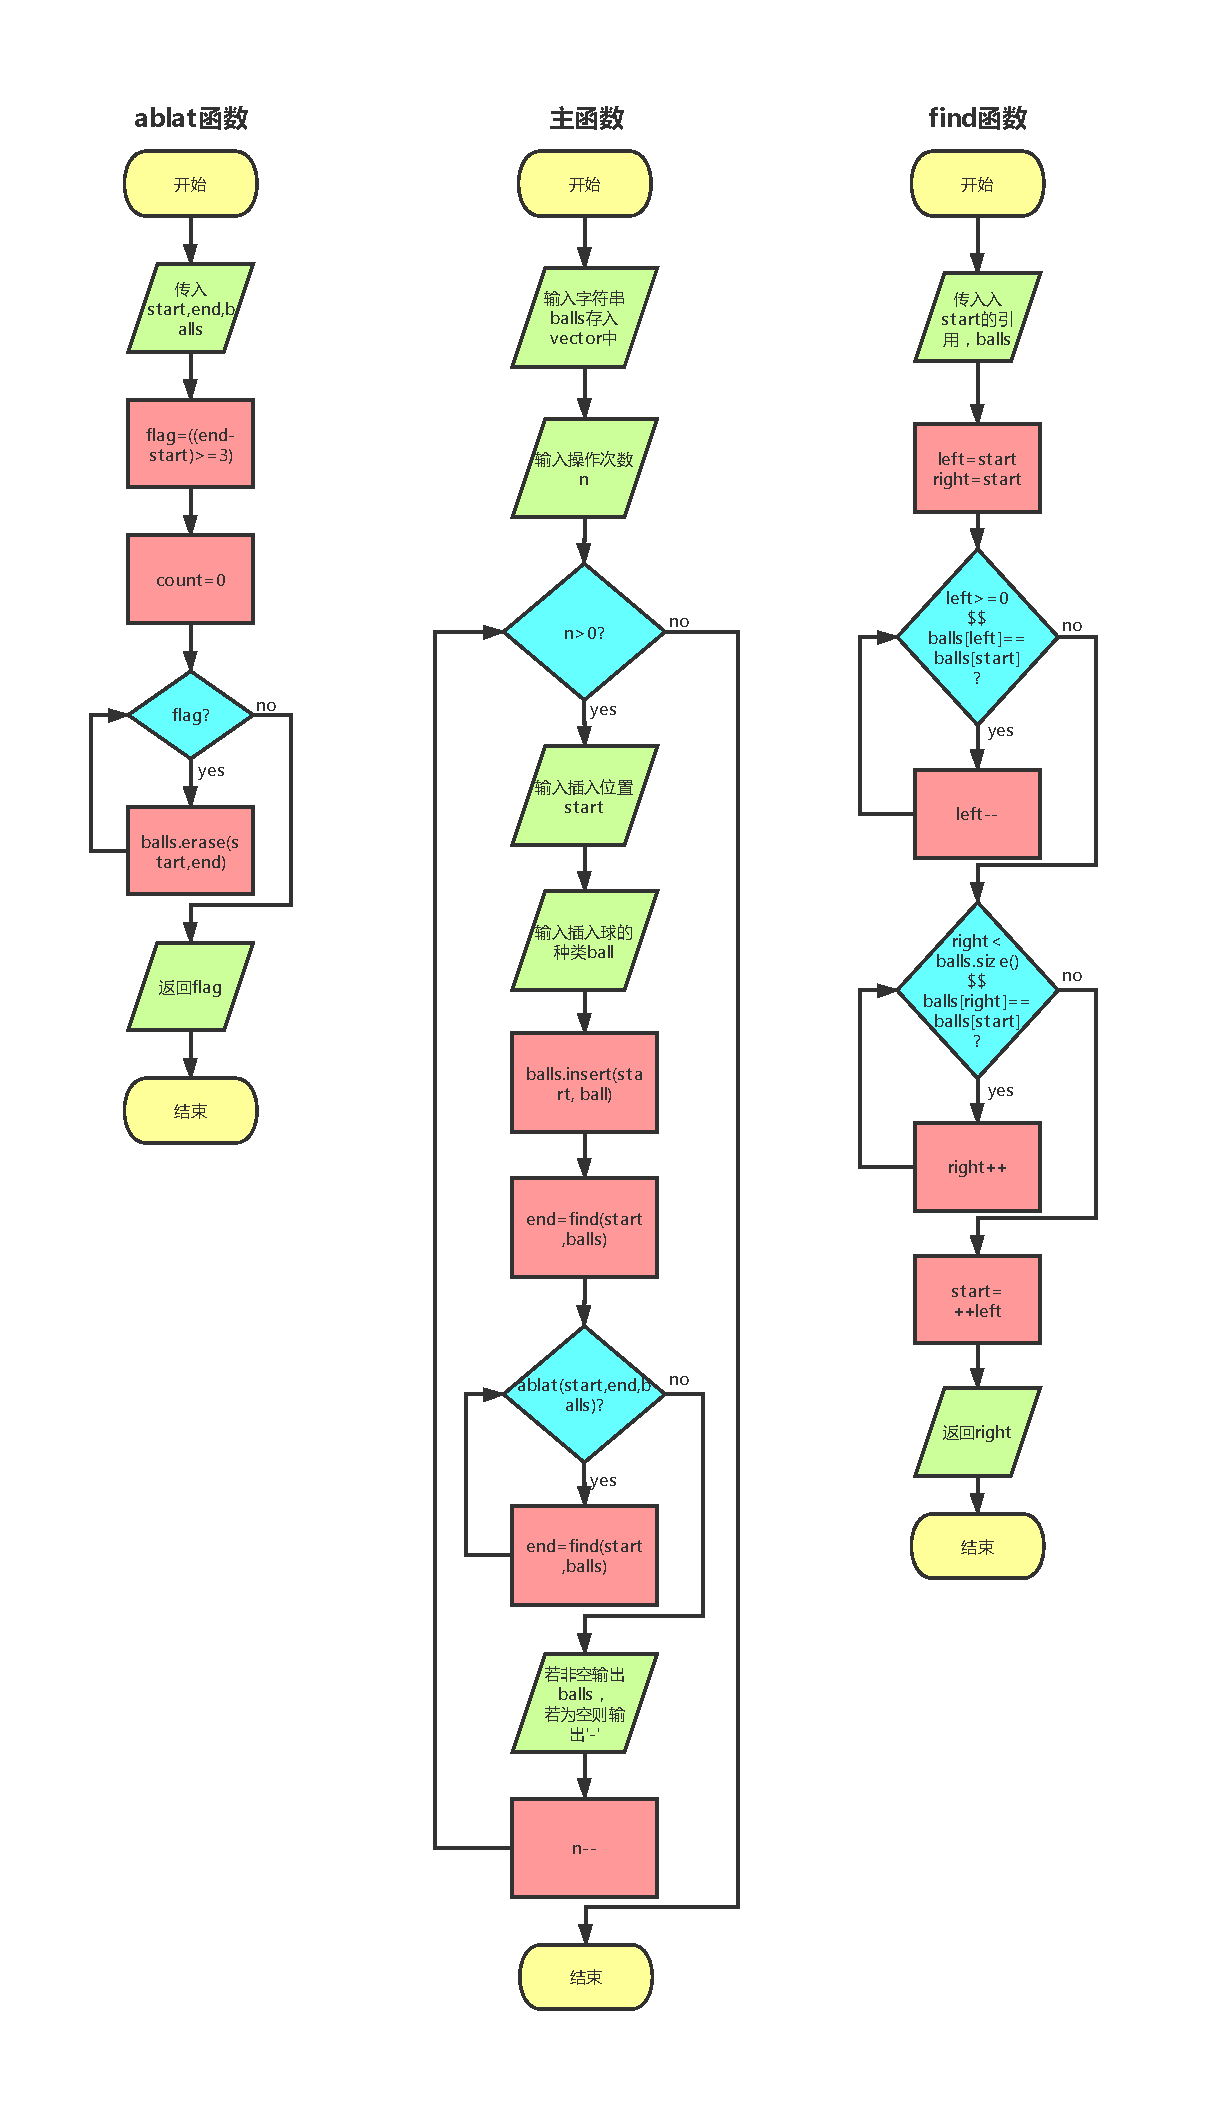
\includegraphics[scale=0.65]{zuma_flowchart.pdf}
%	\caption{vector版流程图}
%	\label{vec_flowchart}
%\end{figure}
%
%\newpage

	\subsection{代码一}
我们两个人写了两段代码,两者都能实现问题。这是第一段代码\footnote{latex编译注释存在中文和英文、数字排序混乱,部分混乱可能是漏加了逃逸字串}
	\begin{lstlisting}[language=C,caption={第一段代码},label={dbl_code}]
#include <iostream>
#include <cstdio>
#include <cstring>
#include <algorithm>
using namespace std;
typedef struct
{
    int weight;                 //权值
    int parent, lchild, rchild; //双亲,左子树,右子树,注意这是一个静态链表
} HTNode, *HuffmanTree;         //结点,指针
void Select(HuffmanTree HT, int x, int &s1, int &s2)
{
    int f = 0, g = 0;            //`初始化f,g,作用相当于flag`
    for (int i = 1; i <= x; i++) //注意满足了一个if就会直接跳到下一个循环
    {
        if (HT[i].parent != 0) //`如果说i结点已经被分配了双亲就跳过它`
        {
            continue;
        }
        if (!f) //`如果f是0,用于初始化s1`
        {
            f = 1;
            s1 = i;
        }
        else if (!g) //`如果g是0,用于初始化s2`
        {
            g = 1;
            s2 = i;
            if (HT[s2].weight < HT[s1].weight) //`保证s2的权值大于s1`
            {
                swap(s1, s2);
            }
        }
        else if (HT[i].weight < HT[s1].weight) //`此时s2和s1最小`
        {
            s2 = s1;
            s1 = i;
        }
        else if (HT[i].weight < HT[s2].weight) //`此时s2和s1最小`
        {
            s2 = i;
        }
    }
    cout << " " << HT[s1].weight << " " << HT[s2].weight << endl;
}
void CreateHuffmanTree(HuffmanTree &HT, int n)
{
    if (n <= 1)
        return;             //`n如果小于等于1,无需建立霍夫曼树`
    int m = 2 * n - 1;      //`m是需要建立的节点数`
    HT = new HTNode[m + 1]; //`分配m+1个空间,0号单元未使用`
    for (int i = 1; i <= m; i++)
    {
        HT[i].parent = 0;
        HT[i].lchild = 0;
        HT[i].rchild = 0; //`一开始都初始化为0`
    }
    for (int i = 1; i <= n; i++)
    {
        cin >> HT[i].weight; //静态链表,输入木头长度
    }
    for (int i = n + 1; i <= m; i++)
    {
        int s1, s2;
        Select(HT, i - 1, s1, s2); //`s1和s2代表权值最小的编号`
        HT[s1].parent = i;
        HT[s2].parent = i;
        HT[i].lchild = s1;
        HT[i].rchild = s2;
        HT[i].weight = HT[s1].weight + HT[s2].weight; //`第i个结点是s1和s2的双亲,权值为s1和s2的和`
    }
}

void readtree(HuffmanTree ht, int n)
{
    for (int i = 2 * n -1; i >=1; i--)
    if(ht[i].lchild && ht[i].rchild){
        printf("切割%d成为%d和%d\n",ht[i].weight, ht[ht[i].lchild].weight, ht[ht[i].rchild].weight);
    }
}

int main()
{
    int n;
    scanf("%d", &n);                 //`n是木头数量`
    HuffmanTree H = new HTNode[100]; //分配空间
    CreateHuffmanTree(H, n);         //建立霍夫曼树
    int sum = 0;
    for (int i = n + 1; i <= 2 * n - 1; i++)
    {
        sum += H[i].weight; //双亲权值相加得到花费
    }
    readtree(H, n);
    cout << sum << endl;
}
	\end{lstlisting}
\subsection{代码二}
\begin{lstlisting}[language=C,caption={第二段代码},label={dbl_code}]
#include <stdio.h>
#include <string.h>
void paixv(int a[], int i, int length) //最小堆排序
{
int mins = i;
int lch = i * 2;
int rch = i * 2 + 1;
if(lch <= length && a[lch] < a[i]) mins = lch;
if(rch <= length && a[rch] < a[mins]) mins = rch;//确定最小值的位置
if(mins != i)
{
int t = a[i];
a[i] = a[mins];
a[mins] = t;                                  //交换位置
paixv(a, mins, length);                       //递归进行
}
}
void buildHd(int a[], int length)//引入最小堆排序
{
for(int i = length / 2; i > 0; i--){
paixv(a,i,  length);            }
}
int pop_head(int a[], int& length)     //POP
{
int t = a[1];
a[1] = a[length];      //把最后一个位置的data放到头上再重新排序
paixv(a,1, --length);
return t;                 //打印出原第一个位置的data
}
void insert_paixv(int a[],int& length, int data ) //入队并排序
{
length++;
a[length] = data;
int i=length;
while(i > 1 && a[i] < a[i / 2])//上浮
{
int t = a[i];
a[i] = a[i / 2];
a[i / 2] = t;
i = i/2;
}
}//把新元素插入到最后然后只排序这一趟
int a[10000] = {0};
int main(){
int n;
scanf("%d",&n);
int length = n;
for(int i = 1; i < n+1; ++i)
{
scanf(" %d", &a[i]);
}
buildHd(a, length);//构建队列
int sum = 0;
while(length > 1){
int x = pop_head(a, length);
int y = pop_head(a, length);//队头两个元素是小的,POP出来
insert_paixv(a, length,x+y);
sum += x+y;
}
printf("%d", sum);
}
\end{lstlisting}
	\subsection{运行结果截图}
\begin{figure}[h]
	\centering
	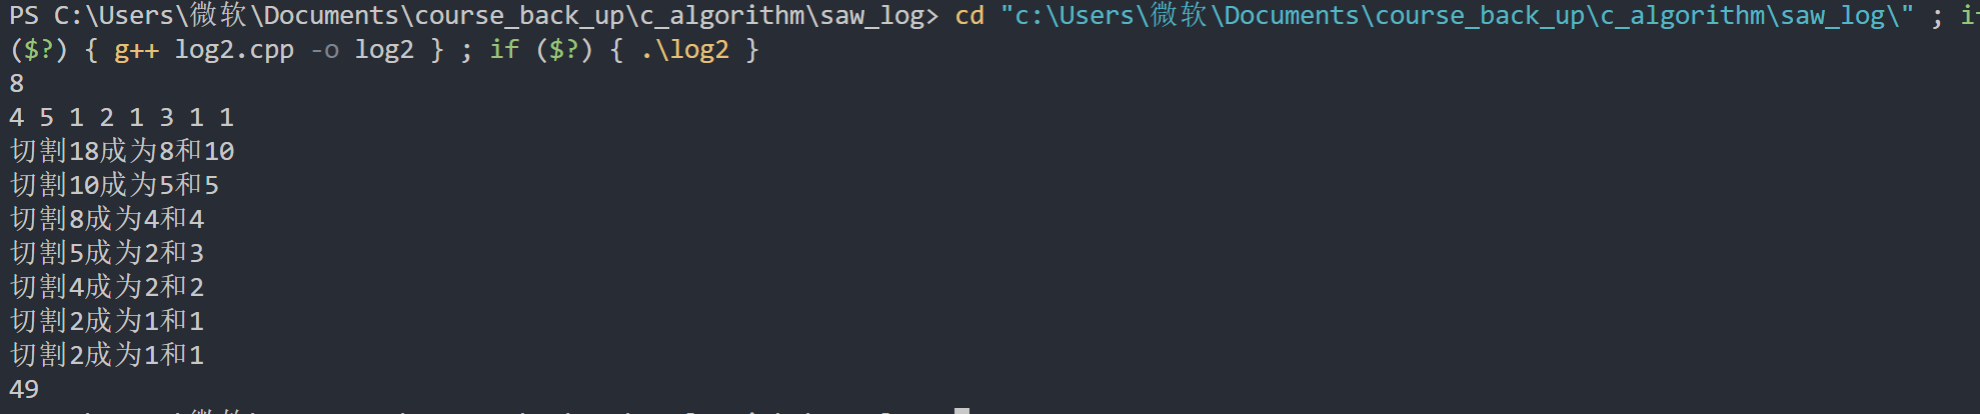
\includegraphics[scale=0.6]{result4.png}
	\caption{运行结果1}
\end{figure}
\begin{figure}[h]
	\centering
	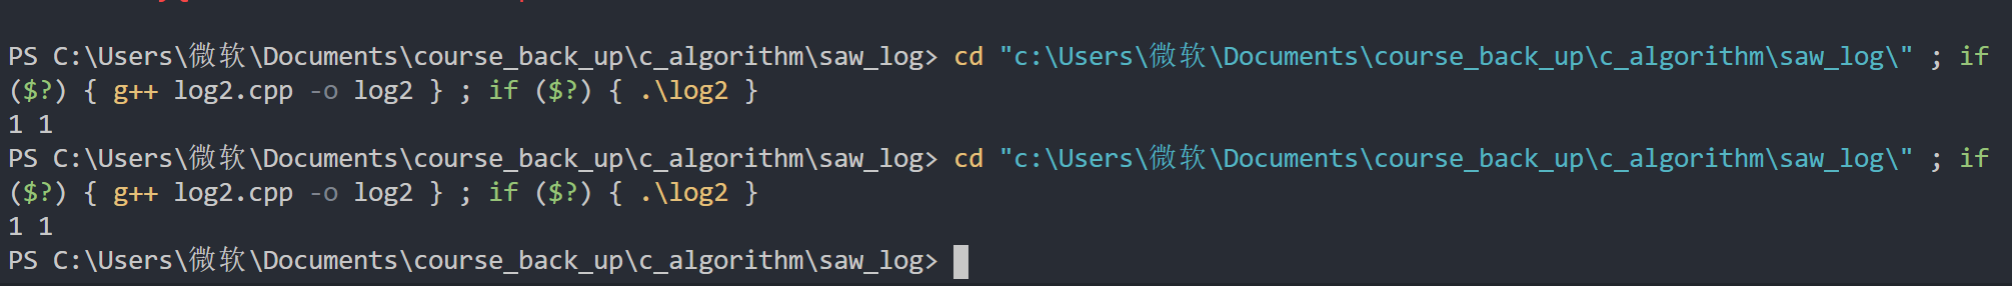
\includegraphics[scale=0.6]{result5.png}
	\caption{运行结果2}
\end{figure}
\begin{figure}[h]
	\centering
	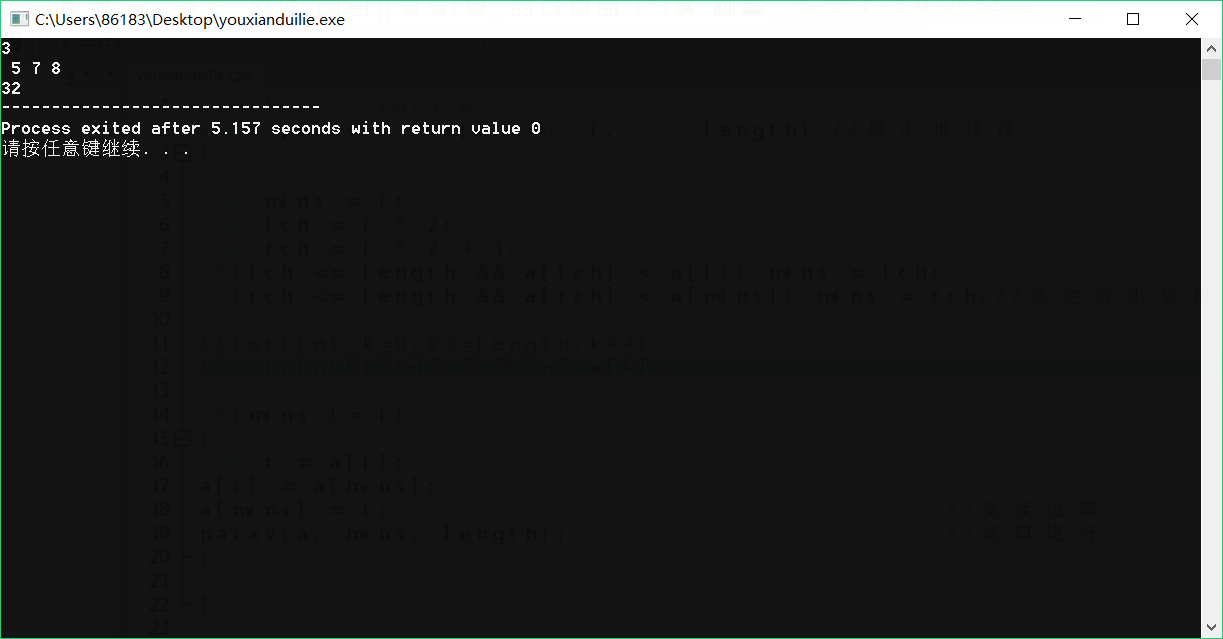
\includegraphics[scale=0.6]{result6.png}
	\caption{运行结果3}
\end{figure}
\begin{figure}[h]
	\centering
	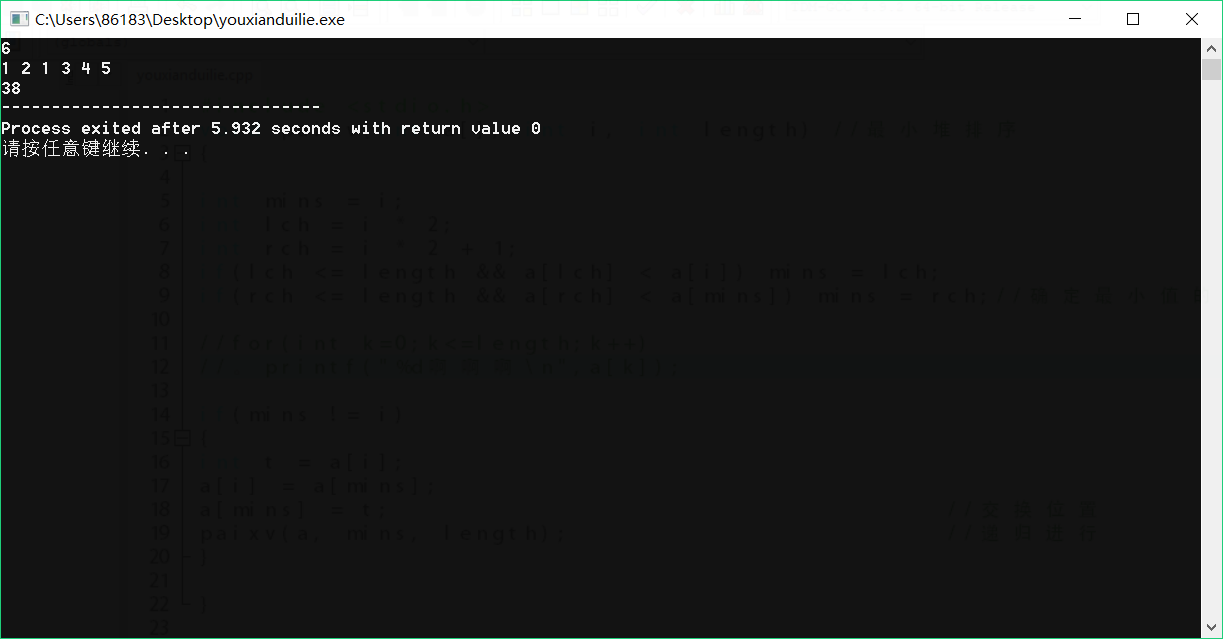
\includegraphics[scale=0.6]{result7.png}
	\caption{运行结果4}
\end{figure}

%	\begin{itemize}
%	\item 输入
%		\begin{itemize}
%			\item[ ]ACCBA
%			\item[ ]5
%			\item[ ]1 B
%			\item[ ]0 A
%			\item[ ]2 B
%			\item[ ]4 C
%			\item[ ]0 A
%		\end{itemize}
%	\item 输出
%		\begin{itemize}
%			\item[ ]ABCCBA
%			\item[ ]AABCCBA
%			\item[ ]AABBCCBA
%			\item[ ]-
%			\item[ ]A	
%		\end{itemize}
%	\end{itemize}
%	
%	\indent 更换多组数据测试均正确,其中$vector$版本以100分的成绩通过清华大学$Open\ Judge$测试。
	\subsection{总结体会}
	\indent 看到这道题,首先想到的就是用冒泡排序,然后把最小的两个合并再依次往上,一个一个的合并,其他的木头,这样就形成了一颗如图$5$所示的二叉树。把所有的非叶子节点求和即可得到最后答案,但是这种考虑忽视了,如图所示$6$的做法,只适用一些特殊的情况。采用优先队列的做法,可以实现对上图这种情况的处理。.通过做这道题可以对堆排序有更深刻的理解,中间的有些想法是在参考了网上的优先队列堆排序的实现之后才想到,过程有一些抽象的地方,有待巩固以熟练掌握。
\begin{figure}[h]
	\centering
	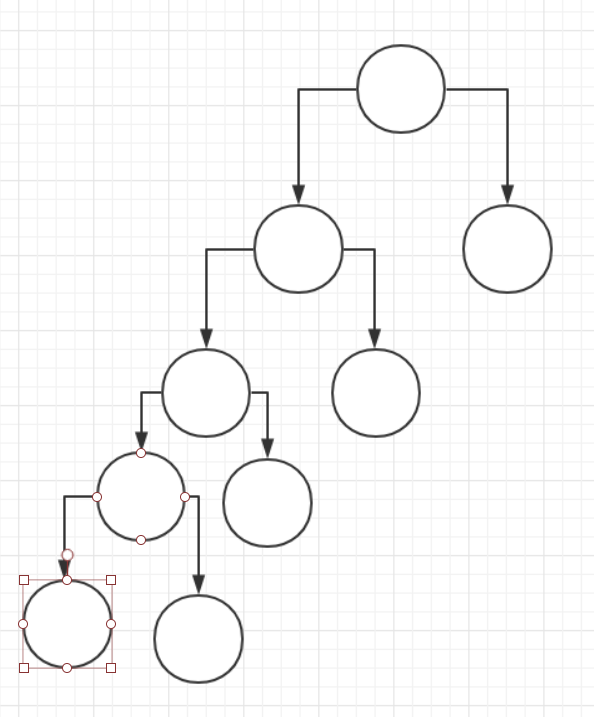
\includegraphics[scale=0.6]{pic3.png}
	\caption{第一次想到的,有遗漏}
\end{figure}
\begin{figure}[h]
	\centering
	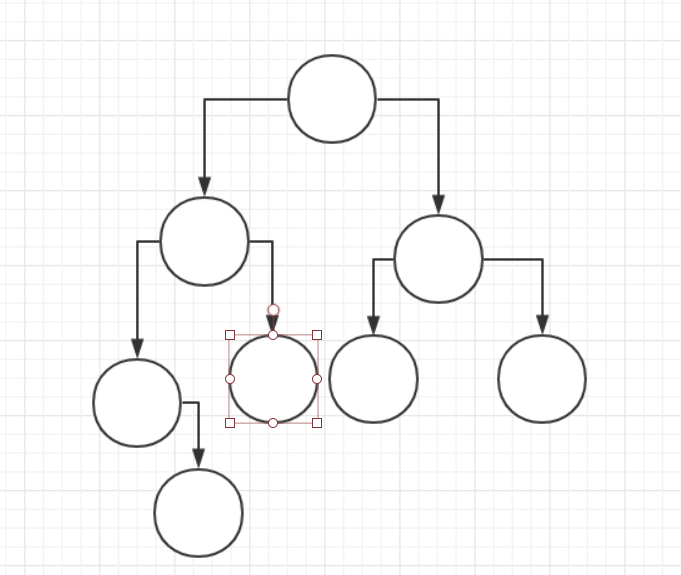
\includegraphics[scale=0.6]{pic4.png}
\caption{最终实现的}
\end{figure}
%\section{第二题}
%\subsection{实验目的和内容}
%	\indent 祖玛是一款曾经风靡全球的游戏,其玩法是:在一条轨道上初始排列着若干个彩色珠子,其中任意三个相邻的珠子不会完全同色。此后,你可以发射珠子到轨道上并加入原有序列中。一旦有三个或更多同色的珠子变成相邻,它们就会立即消失。这类消除现象可能会连锁式发生,其间你将暂时不能发射珠子。
%
%\indent 开发商最近准备为玩家写一个游戏过程的回放工具。他们已经在游戏内完成了过程记录的功能,而回放功能的实现则委托你来完成。
%
%\indent 游戏过程的记录中,首先是轨道上初始的珠子序列,然后是玩家接下来所做的一系列操作。你的任务是,在各次操作之后及时计算出新的珠子序列。
%\subsection{输入和输出说明}
%	\subsubsection{输入}
%	\indent 第一行是一个由大写字母$’A’~’Z’$组成的字符串,表示轨道上初始的珠子序列,不同的字母表示不同的颜色。
%
%\indent 第二行是一个数字$n$,表示整个回放过程共有$n$次操作。
%
%\indent 接下来的$n$行依次对应于各次操作。每次操作由一个数字$k$和一个大写字母$\sum$描述,以空格分隔。其中,$\sum$为新珠子的颜色。若插入前共有$m$颗珠子,则$k\in[0, m]$表示新珠子嵌入之后(尚未发生消除之前)在轨道上的位序。
%	\subsubsection{输出}
%	\indent 输出共$n$行,依次给出各次操作(及可能随即发生的消除现象)之后轨道上的珠子序列。
%
%\indent 如果轨道上已没有珠子,则以“$-$”表示。
%	\subsubsection{样例}
%	\begin{itemize}
%	\item 输入
%		\begin{itemize}
%			\item[ ]ACCBA
%			\item[ ]5
%			\item[ ]1 B
%			\item[ ]0 A
%			\item[ ]2 B
%			\item[ ]4 C
%			\item[ ]0 A
%		\end{itemize}
%	\item 输出
%		\begin{itemize}
%			\item[ ]ABCCBA
%			\item[ ]AABCCBA
%			\item[ ]AABBCCBA
%			\item[ ]-
%			\item[ ]A	
%		\end{itemize}
%	\end{itemize}
%\subsection{解题思路}
%本题主要用了五个函数。\par
%第一个建立双向链表函数,定义了头指针和尾指针并赋值$'-'$,并且用数组传参\par
%第二个插入函数,就是找到某一个位置并进行插入\par
%第三个是找到双向链表尾部,这个函数为删除,输出函数铺垫\par
%第四个删除函数,需要注意的有两点:
%\begin{itemize}
%  \item 第一是需要找准删除的起点和终点
%  \item 第二是需要讨论三种及以上的球的情况
%\end{itemize}
%第五个是输出函数,我们将双向链表赋值给数组并输出
%
%\subsection{实验代码及注释}
%\begin{lstlisting}
%#include <stdio.h>
%#include "string.h"
%#include <stdlib.h>
%#include <malloc.h>
%
%#define Len 20000
%#define Up (Len * 3 / 4)
%
%typedef char ElemType;
%typedef struct node //定义双向链表
%{
%    ElemType data; //数据域
%    struct node *next;
%    struct node *front; //指针域
%} List, *pList;         //结点类型,结点指针
%
%// pList pHead = (pList)malloc(sizeof(List));
%// pList pTail = (pList)malloc(sizeof(List));
%//常量表达式中不允许函数调用
%
%char ans[Len + 5];
%int forprt = 0;
%
%pList creat(char *a, int n)
%{
%    /* n为参数个数,*a为传入参数*/
%    int i;
%    pList pHead = (pList)malloc(sizeof(List));
%    pList pTail = (pList)malloc(sizeof(List)); //创建头指针和尾指针
%
%    pList pt = pHead; // pt指向头指针
%
%    pTail->front = pHead;
%    pTail->next = NULL;
%    pHead->next = pTail;
%    pHead->front = NULL;             //创建空的双向链表
%    pHead->data = pTail->data = '-'; //赋值为'-',表示轨道上已没有珠子
%
%    for (i = 0; i < n; i++)
%    {
%        pList pNew = (pList)malloc(sizeof(List));
%        pNew->data = a[i];  // 先通过gets得到数组储存字符串,然后通过数组来传值
%        pNew->front = pt;
%        pNew->next = pt->next;
%        pt->next->front = pNew;
%        pt->next = pNew;
%        pt = pNew;  //移动pt指针
%    }
%    return pHead;
%}
%
%pList insert(int m, char ch, pList pHead)
%{
%    int i = -1; // i=-1.方便对位置零操作
%
%    pList pt = pHead, pNew = (pList)malloc(sizeof(List));
%
%    while (i++ < m)
%        pt = pt->next; //找到带插入位置
%
%    pNew->data = ch;
%    pNew->next = pt;
%    pNew->front = pt->front;
%    pt->front->next = pNew;
%    pt->front = pNew; //注意是插在找到位置的前面
%
%    return pHead;
%}
%
%pList find_tail(pList pHead)
%{
%    pList pt = pHead->next;
%    //while(!(pt->data == '-')) pt = pt ->next;
%    while (pt->next != NULL)
%        pt = pt->next;   //这两种方法都可以找到pTail
%    return pt;
%}
%
%pList del(int m, pList pHead)
%{
%    pList pTail, point_tmp;
%    pTail = find_tail(pHead);
%    //获得ptail
%    pList p1 = NULL, p2 = NULL, p3 = NULL, p4 = NULL, pt = pHead; //空指针最好赋值 NULL
%    pList begin = pHead, end = pTail;
%    int boo = 1; //gcc编译器不支持bool类型,所以用int表示逻辑
%    int repeat, i = -1;
%
%    // find position
%    while (i++ < m - 2)
%        pt = pt->next; // 找到插入位置前两个指针
%
%    //init for 'begin' and 'end'
%    begin = pt;
%    end = pt;
%    i = 0;
%    while (i++ < 4 && end->next != pTail)
%        end = end->next; //找到插入位置后两个指针
%
%    while (boo && pt != pTail)
%    {
%        boo = 0; //判断有没有发生消除
%        repeat = 1; //计数重复的个数
%        while (pt != end) //pt在begin位置
%        {
%            pt = pt->next;
%
%            if (pt->front->data == pt->data) //pt后移,如果data相同,就计数加一
%                repeat++;
%            else
%                repeat = 1;
%
%            if (repeat == 3)
%            {
%                boo = 1;
%                if (pt->data == pt->next->data) //已经满足消除条件了,再看看能不能继续满足
%                {
%                    repeat++;
%                    pt = pt->next;
%                }
%
%                if (repeat == 3)
%                {
%                    p3 = pt;
%                    p2 = p3->front;
%                    p1 = p2->front;
%                    p1->front->next = p3->next;
%                    p3->next->front = p1->front;
%                    pt = pt->next; //消除这三个,将pt后移
%                    free(p1);
%                    free(p2);
%                    free(p3);
%                }
%                else
%                {
%                    p4 = pt;
%                    p3 = p4->front;
%                    p2 = p3->front;
%                    p1 = p2->front;
%                    p1->front->next = p4->next;
%                    p4->next->front = p1->front;
%                    pt = pt->next; //消除这4个,将pt后移
%                    free(p1);
%                    free(p2);
%                    free(p3);
%                    free(p4);
%                }
%
%                break;
%            }
%        }
%
%        if (boo && pt != pTail)
%        {
%            begin = pt;
%            i = 0;
%            while (i++ < 2 && begin->front != pHead)
%                begin = begin->front;
%            end = pt;
%            i = 0;
%            if (i++ < 1 && end->next != pTail)
%                end = end->next;
%            pt = begin; //将pt的begin和end指针归位
%        }
%    }
%    return pHead;
%}
%
%pList show(int boo, pList pHead) //将双向链表的值存到数组便于输出
%{
%
%    pList pt = pHead->next;
%    pList pTail = find_tail(pHead);
%
%    if (pt == pTail)
%        ans[forprt++] = '-'; //没有数
%    else
%    {
%        while (pt->next != NULL)
%        {
%            ans[forprt++] = pt->data; //扩容并存data
%            pt = pt->next;  //pt后移
%        }
%    }
%
%    ans[forprt++] = '\n'; //输出需要有换行
%
%    if (forprt >= Up || boo) //如果到尽头了
%    {
%        ans[forprt] = '\0'; //数组一定要以 \0 结尾
%        printf("%s", ans); //输出
%        forprt = 0;
%    }
%    return pHead; //其实不需要返回了
%}
%
%int main(void)
%{
%    char a[10005];
%    int n, k;
%    pList pHead = NULL;
%
%    //printf("请输入初始队列\n");
%    gets(a); // 初始的珠子序列
%    //printf("请输入操作数");
%    scanf("%d", &n); // 共有n次操作
%
%    pHead = creat(a, strlen(a)); //创建对应初始的珠子序列的双向链表
%
%    for (k = 0; k < n; k++)
%    {
%        int m;
%        char ch;
%
%        scanf("%d ", &m); //新的珠子位序
%
%        ch = getchar(); // 插入珠子颜色
%
%        // insert ch
%        insert(m, ch, pHead);
%
%        // delete all 3-same block, making it the right string
%        del(m, pHead);
%
%        // print the string
%        show(k == n - 1 ? 1 : 0, pHead);
%    }
%
%    return 0;
%}
%\end{lstlisting}
%\subsection{运行结果截图}
%%\begin{figure}[!htbp]
%%	\centering
%%	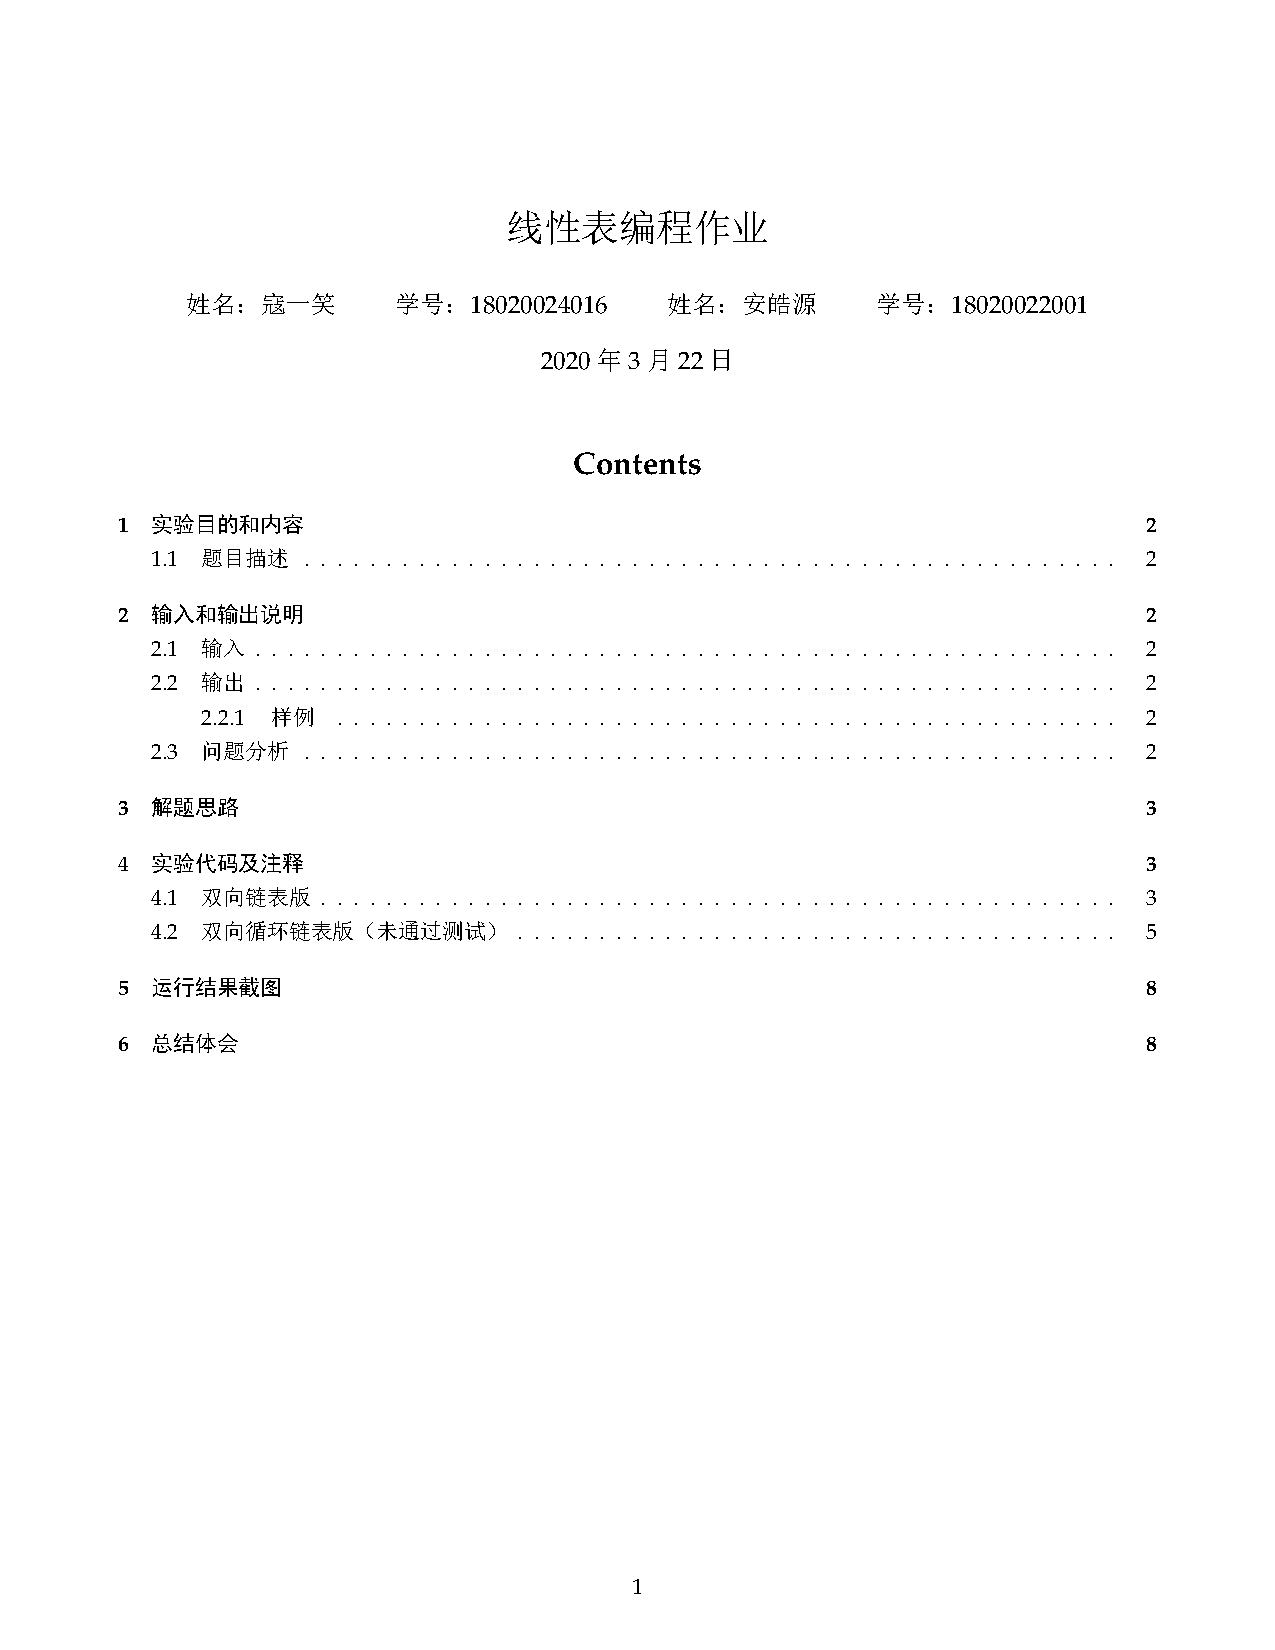
\includegraphics[scale=0.65]{zuma.png}
%%	\caption{运行结果}
%%\end{figure}
%\subsection{总结体会}
%主要复习了debug的基本操作,熟悉了双向链表的建立和删除操作。同时对于“实际问题”,需要分类讨论,考虑到多种情况。对于一些重复利用的操作可以写成函数方便调用
%\bibliography{ref.bib}
\end{document} 